\section{ChimeraX Rigid Fit protocol}
\label{app:chimeraRigidFit}%a040
Protocol designed to manually fit atomic structures to electron density maps in \scipion by using \chimera. If \iii{map} and \iii{model} are quite close, e.g. after running \phenix \ttt{dock in map} protocol, automatic fitting is also possible. Fitted atomic structures generated by using this protocol can be saved in \scipion after executing specific \chimera commands.
   
 \begin{itemize}
  \item Requirements to run this protocol and visualize results:
    \begin{itemize}
    \item \scipion plugin: \ttt{scipion-em}
        \item \scipion plugin: \ttt{scipion-em-chimera}
    \end{itemize}
  \item \scipion menu:\\
   \ttt{Model building -> Rigid fitting} (\ffigure{fig:app_protocol_chimera_1} (A))
  
  \item Protocol form parameters (\ffigure{fig:app_protocol_chimera_1} (B)):
  
    \begin{figure}[H]
     \centering 
     \captionsetup{width=.9\linewidth} 
     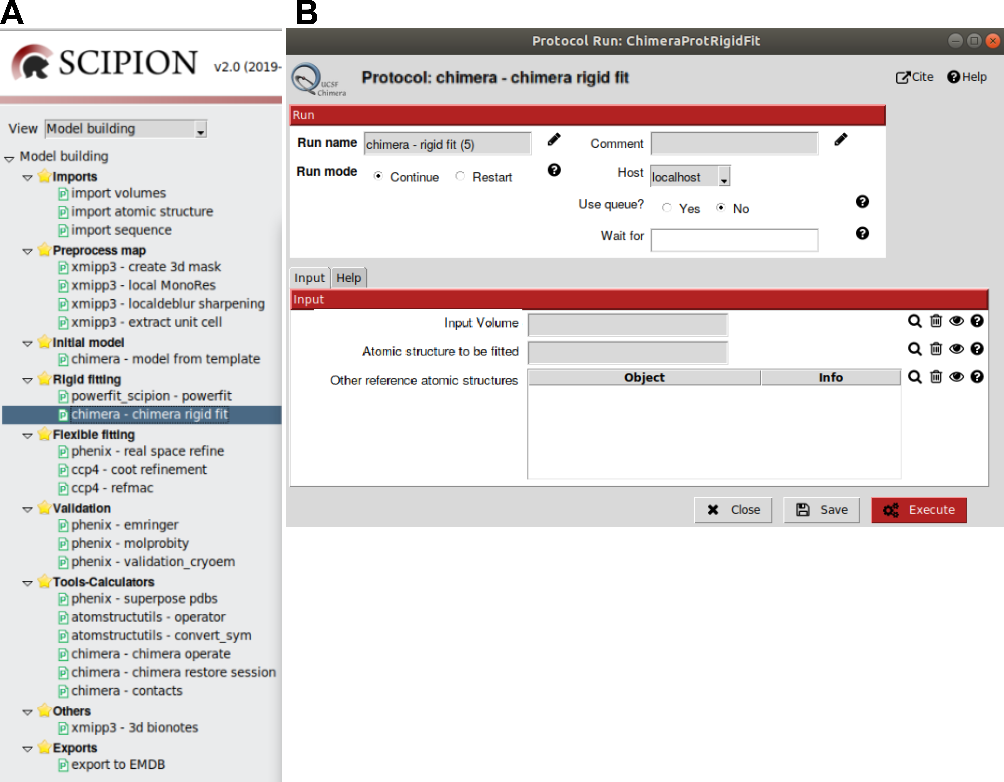
\includegraphics[width=0.90\textwidth]{Images_appendix/Fig116.pdf}
     \caption{Protocol \scommand{chimerax - rigid fit}. A: Protocol location in \scipion menu. B: Protocol form.}
     \label{fig:app_protocol_chimera_1}
    \end{figure}
    
    \begin{itemize}
     \item \ttt{Input} section

    \begin{itemize}
     \item \ttt{Input Volume}: Mandatory param to load the electron density \iii{map} previously downloaded or generated in \scipion to fit the atomic structure.
     \item \ttt{Input Volume}: $Idem$. If additional maps, others than the previous \iii{map}, are needed.
     \item \ttt{Atomic structure to be fitted}: Mandatory param to load the atomic structure previously downloaded or generated in \scipion to be fitted to an electron density map.
     \item \ttt{Other reference atomic structures}: Atomic structures others than the \iii{model} that can help in the rigid body fitting process.
    \end{itemize}
    \item \ttt{Help} section
    
    This section contains \chimera commands required to save \iii{models} according to their reference volumes, which can also be saved if required. Remark that using \ttt{scipionwrite} command, \chimera session will be saved by default, without prejudice that it may be saved with \ttt{scipionss} command. \chimera sessions can be restored by using \scommand{chimerax - restore session} protocol. In addition \ttt{scipioncombine} allows to combine several atomic structures in a unique \iii{model}.
    
    \end{itemize}

  \item Protocol execution:
  
  Adding specific map/structure label is recommended in \ttt{Run name} section, at the form top. To add the label, open the protocol form, press the pencil symbol at the right side of \ttt{Run name} box, complete the label in the new opened window, press OK and, finally, close the protocol. This label will be shown in the output summary content (see below). If you want to run again this protocol, do not forget to set to \ttt{Restart} the \ttt{Run mode}.\\
  Press the \ttt{Execute} red button at the form bottom.\\
  
  \chimera graphics window will be opened after executing the protocol. The electron density map and the atomic structure are shown. Main steps to complete the rigid body fitting are:
  \begin{itemize}
   \item If density map and atomic structure are quite close to each other:\\Go to \chimera main menu and select \ttt{Tools -> Volume Data-> Fit in Map}. A small \ttt{Fit in Map} window will be opened. Once the right atomic structure and the electron density volume have been selected, fit them by clicking \ttt{Fit}.\\
   \ttt{Note}: The same result can be obtained by typing in the command line \ttt{fitmap \#n1 inMap \#n2}, with \ttt{\#n1} and \ttt{\#n2} \chimera model numbers of \iii{model} and \iii{map}.
   \item If \iii{model} and \iii{map} are far from each other, start the fitting process interactively activating and inactivating \chimera objects alternatively to finally get \iii{map} and \iii{model} close enough to go to the previous step. Otherwise, consider the possibility of running before the \phenix \ttt{dock in map} protocol.
   \item To combine two or more atomic structures:\\
                            Write in \chimera command line:\\
                            \ttt{scipioncombine \#n1,n2}\\
                            \\
                            \ttt{\#n1} and \ttt{\#n2} are the respective $model$ numbers of two different atomic structures. Optionally you can set the $model$ number of the output combined structure \ttt{\#n3}:\\
                            \ttt{scipioncombine \#n1,n2 modelid n3}\\
   \item Save fitted \iii{model} regarding the \iii{map} by writing in \chimera command line:\\ \ttt{scipionwrite \#n prefix userString\_}.\\Replace \ttt{\#n} by model numbers shown in \chimera \ttt{Models} panel. \ttt{prefix} + string preferred by the user to easily identify the atomic structure is optional, although quite recomendable.
   \item Close \chimera graphics window.
  \end{itemize}
  
  \item Visualization of protocol results:
  
    After executing the protocol, press \ttt{Analyze Results} and \chimera graphics window will be opened by default. Atomic structures and volumes are referred to the origin of coordinates in \chimera. To show the relative position of \iii{model} and \iii{map}, the three coordinate axes are represented; X axis (red), Y axis (yellow), and Z axis (blue) (\ffigure{fig:app_protocol_volume_3}). Coordinate axes, map, and atomic structure are model numbers \ttt{\#1}, \ttt{\#2}, and \ttt{\#3}, respectively, in \chimera \ttt{Models} panel in the most simple case.
   
  \item Summary content:
   \begin{itemize}
    \item If only the atomic structure has been saved by \ttt{scipionwrite} command:

   \begin{itemize}
     \item Protocol output (below \scipion framework):\\
                                        \ttt{chimerax - operate -> output atomic structure name, starting with the prefix};\\ \ttt{AtomStruct (pseudoatoms=True/ False, volume=True/ False)}.\\Pseudoatoms is set to \ttt{True} when the structure is made of pseudoatoms instead of atoms. Volume is set to \ttt{True} when an electron density map is associated to the atomic structure.
                                \item \ttt{SUMMARY} box:\\Produced files:\\output atomic structure name, starting with the prefix (.cif file)\\we have some result
    \end{itemize}
    
   \item If both the atomic structure and its reference electron density map have been saved by \ttt{scipionwrite} command: 
   
   \begin{itemize}
     \item Protocol output (below \scipion framework):\\
      \ttt{chimerax - rigid fit -> Map\_name}; \ttt{Volume (x, y, and z dimensions, sampling rate)}.\\
      \ttt{chimerax - rigid fit -> Atom\_struct\_name};\\ \ttt{AtomStruct (pseudoatoms=True/ False, volume=True/ False)}.\\Pseudoatoms is set to \ttt{True} when the structure is made of pseudoatoms instead of atoms. Volume is set to \ttt{True} when an electron density map is associated to the atomic structure.
     \item \ttt{SUMMARY} box:\\Produced files:\\Map\_name file, starting with the prefix (.mrc)\\we have some result
    \end{itemize}
    
   \end{itemize} 
  
 \end{itemize}

